% !TEX TS-program = xelatex
% !TEX encoding = UTF-8
%
%
\documentclass[a4paper,12pt]{article}
\usepackage{ctex}
\usepackage{geometry,anysize,changepage,calc,hyperref,cite,fancyhdr,setspace}
\usepackage{amsmath,amssymb,amsthm,listings,xcolor}
\usepackage{graphicx,wrapfig,multirow,diagbox,caption, subcaption,verbatim}
\usepackage{caption,algorithm,algpseudocode}
\usepackage{url,natbib}
\bibliographystyle{abbrvnat}
\setcitestyle{open={(},authoryear,close={)}}
\renewcommand{\algorithmicrequire}{\textbf{输入}}
\renewcommand{\algorithmicensure}{\textbf{输出}}
\floatname{algorithm}{子程序}
\listfiles
%initialset.tex
%
\hypersetup{bookmarksopen=true,colorlinks=true,linkcolor=red,anchorcolor=blue,citecolor=green,linktocpage=true}
\captionsetup{font=footnotesize}
\captionsetup[sub]{font+=footnotesize}
\linespread{1.5}
\marginsize{2.13cm}{2.14cm}{2.4cm}{2.4cm}
\pagestyle{fancy}
\lstset{xleftmargin=1.5em,xrightmargin=1.5em,frame=lines}%,numbers=left,numberstyle=\tiny}
\chead{}\rhead{\thepage}\lhead{\leftmark}\cfoot{}\rfoot{}\lfoot{}

\newcommand{\vp}{\varphi}
\newcommand{\al}{\alpha}
\newcommand{\be}{\beta}
\newcommand{\ti}{\tilde}
\newcommand{\ve}{\varepsilon}
\newcommand{\de}{\delta}
\newcommand{\na}{\nabla}
\newcommand{\pd}{\partial}
\newcommand{\ud}{\mathrm{d}}
\newcommand{\mr}{\mathrm{R}}
\newcommand{\ms}{\mathbb{S}}
\newcommand{\mz}{\mathbb{Z}}
\newcommand{\mn}{\mathbb{N}}
\newcommand{\mc}{\mathbb{C}}
\newcommand{\one}{\textbf{1}}
\newcommand{\prox}{\textbf{prox}}
\DeclareMathOperator*{\argmax}{argmax}
\DeclareMathOperator*{\argmin}{argmin}
%\DeclareMathOperator*{\logg}{log}
%\DeclareMathOperator*{\det}{det}
\DeclareMathOperator*{\tr}{tr}
\DeclareMathOperator*{\st}{s.t.}

\theoremstyle{nonumberplain}
%\theoremheaderfont{\itshape}
%\theorembodyfont{\upshape}
%\theoremseparator{.}
%\theoremsymbol{\ensuremath{\square}
\newtheorem{definition}{定义}
\newtheorem{theorem}{定理}
\newtheorem{lemma}{引理}
%\newtheorem{proof}{证明}

%\renewcommand{\figurename}{{\zihao{5}图}}
%\renewcommand{\tablename}{{\zihao{5}表}}
%\makeatletter %下面两个命令用于创建非浮动体图表的标题
%  \newcommand\figcaption{\def\@captype{figure}\caption} 
%  \newcommand\tabcaption{\def\@captype{table}\caption} 
%\makeatother
%%\renewcommand{\abstractname}{摘\ 要}
%\renewcommand{\contentsname}{目\ 录}
%\renewcommand{\refname}{参考文献}

%\renewcommand{\thetable}{\arabic{section}.\arabic{table}}
%\renewcommand{\thefigure}{\arabic{section}.\arabic{figure}}
%\renewcommand{\theequation}{\arabic{section}.\arabic{equation}}

\makeatletter\@addtoreset{table}{section}\@addtoreset{figure}{section}\@addtoreset{equation}{section}\makeatother




\linespread{1.5}
\author{龙子超}
\title{{\heiti {\zihao{3} 数学分析II-习题课}}}
\date{}
\begin{document}
\maketitle
%===================正文====================
%\begin{abstract}
%\begin{spacing}{1.0}
%
%\end{spacing}
%\end{abstract}

%\tableofcontents
%\newpage

本习题答案集所给出的解答尽可能从教材出发. 课程教材为《数学分析》I-III, 伍胜健编著,
北京大学出版社.
\section*{2018-Feb-28}
\noindent 3. 设函数 $f(x)\in C([0,1])$ 且 $f(0)\neq f(1)$. 
证明: 存在 $\xi\in(0,1)$ 不是 $f(x)$ 的极值点.
  \begin{proof}
(若在考试中下面的证明过程应该更规范): 不失一般性,
我们考虑 $f(0)<f(1)$ 的情形, 记 $a_0=0,b_0=1$, 依题设有 $f(a_0)<f(b_0)$. 
我们构造如下$\{a_n\}_n,\{b_n\}_n$
\begin{algorithm}
  \begin{algorithmic}
    \State for $n=0,1,\cdots$
    \State \ \ \ \ find $x\in(a_n,b_n)$ s.t. $f(x)=\frac{f(a_n)+f(b_n)}{2}$
    \State \ \ \ \ if $x-a_n<b_n-x$
    \State \ \ \ \ \ \ \ \ find $y\in(a_n,x)$ s.t. $f(y)=\frac{f(a_n)+f(x)}{2}$
    \State \ \ \ \ else 
    \State \ \ \ \ \ \ \ \ find $y\in(x,b_n)$ s.t. $f(y)=\frac{f(x)+f(b_n)}{2}$
    \State \ \ \ \ set $a_{n+1}=\min(x,y),b_{n+1}=\max(x,y)$
  \end{algorithmic}
\end{algorithm}

容易证明
\begin{eqnarray*}
  &[1]&f(b_0)>f(b_1)>\cdots>f(b_n)>\cdots>\cdots>f(a_n)>\cdots>f(a_1)>f(a_0),\\
  &[2]&b_0>b_1>\cdots>b_n>\cdots>\cdots>a_n>\cdots>a_1>a_0,\\
  &[3]&|a_{n+1}-b_{n+1}|<\frac{|a_n-b_n|}{2}
\end{eqnarray*}
依据闭区间套定理, 存在$c$满足$a_n<c<b_n,\forall n\in \mn$, $\lim_n a_n=\lim_n b_n=c$, 
这时根据$f$的连续性有$f(c)=\lim_n f(a_n)=\lim_nf(b_n)$, 从而进一步有
\[
  f(b_0)>f(b_1)>\cdots>f(b_n)>\cdots>f(c)>\cdots>f(a_n)>\cdots>f(a_1)>f(a_0),\\
\]

依据$c,f(c)$的上述性质可知$c$不是极值点.
  \end{proof}

\noindent 4. 设函数 $f(x)$ 在 $[a,b]$ 内任一点处的极限均为0. 问: $f(x)$ 在 $[a,b]$ 上可积吗?\\
\begin{proof}[提示]
\begin{enumerate}
  \item 先证明$\forall \varepsilon>0,$ 只存在有限个点 $x\in[a,b]$ 使得 $|f(x)|>\varepsilon$.\\
    若有无穷个这样的点$\Rightarrow$那么这些点会有聚点$\Rightarrow$这个聚点处的函数极限非0, 与题设条件矛盾.\\
    备注: 有限闭集中的无穷个点必有聚点--这可由有限覆盖定理证明--而有限覆盖定理可由闭区间套定理证明--
    闭区间套定理可由数列极限中的若干基本性质得到.\\
    经\textbf{同学}提醒, 可以直接用有限覆盖定理证明: 每个点有一个领域, 
    在这个领域内函数绝对值小于$\varepsilon\Rightarrow$由有限覆盖定理, 
    可以用有限个这样的领域覆盖$[a,b]$$\Rightarrow$
    只有有限个点(那些领域的中心才有可能)$x$可能使得$|f(x)|>\varepsilon$
  \item 再依据积分的定义或者达布理论可以证明这个函数黎曼可积. \\
    上面第一步得到结论实际上已经得到了 $f$ 在区间各局部的振幅的性质, 
    此时可以用书中的定理7.2.6直接得到题目的证明, 当然书中的定理7.2.6也是来自于达布理论, 
    来自于黎曼可积的定义.
\end{enumerate}
\end{proof}

\noindent \textbf{5.} 函数作图:
\[
x = \frac{t^3-t^2+2}{t}, 
y = \frac{t^3-1}{t+1}
\]
\begin{figure}[htbp]
  \centering
  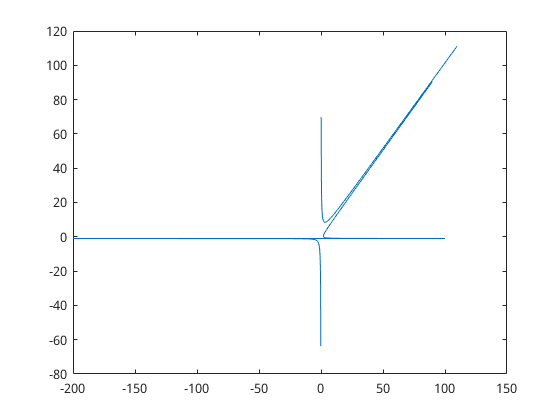
\includegraphics[width = 0.5\textwidth]{20180228_5.png}
  \caption{}
  \label{}
\end{figure}

\noindent \textbf{7.} 设函数 $f(x)$ 在 $x=0$ 处满足 
$f(x)=a_0+a_1x+\cdots+a_nx^n+o(x^n),x\to 0,n\geq1$. 
问: $f(x)$ 在 $x=0$ 处是否存在直至 $n$ 阶导数? 若存在,请计算相应导数值.\\
提示: 取$f(x)=x^{n+1}\sin\frac{1}{x^{n+2}}$分$n=1$和$n>1$讨论.
这个示例函数在0处没有二阶导, 它由一个控制量级的函数$x^{n+1}$
和一个高度震荡但有界的函数$\sin\frac{1}{x^{n+2}}$组成.

\noindent \textbf{8.} 设 $f(x)$ 是 $R$ 上的可微非常值函数且满足 $\forall x\in R, f(f(x))=f(x)$. 
问: $f(x)\equiv x$ 是否成立?
\begin{proof}[证明(by 陈代超)]
  注意到, 对某个 $y\in \mr$, 若存在 $x\in \mr$满足$f(x)=y$, 
则有$f(y)=f(f(x))=f(x)=y$. 因此, $f$的值域中的点都是满足条件的点.

我们只需要证明$f$的值域是$R$.
又由于$f$是连续函数, 因此只需要证明$f$的值域没有上界和下界.\\
以上界为例, 假设$f$有上界, 那么$f$有上确界
\footnote{上确界,下确界是个很好用的概念}, 
我们把它的上确界记作$M$, 并可取$\{x_n\}_n,n=0,1,\cdots$满足$f(x_n)\to M$. 
依题设, $f$不是常值函数, 我们可以取$m<M$,
属于$f$的值域, 因此有$f$的连续性, $[m,f(x_n)]$包含于$f$的值域, 
故其中的任一点$y$都满足$f(y)=y$, 从而$\forall y\in [m,M=\lim_nf(x_n))$, 有$f(y)=y$.
再由于$f$的连续性, 可得$f(M)=M$. 

由于$f(x)=x,x\in[m,M]$, 故$f$的左导数为1, 因此由$f$的可微性, 可知$f$的右导数也为1. 
于是, 存在$\{x'_n\}_n$满足
\begin{eqnarray*}
  &&x'_n\to M, x'_n>M\\
  &&\lim_{n\to\infty}\frac{f(x'_n)-f(M)}{x'_n-M}=1
\end{eqnarray*}
取一个这样的$x'_N$满足$f(x'_N)-f(M)>\frac{x'_n-M}{2}>0$, 则有$f(x'_N)>f(M)=M$, 
这与$M$是$f$值域的上确界矛盾.

因此$f$值域无上界, 同理, $f$值域无下界. 证毕.
\end{proof}

\noindent \textbf{9.} 设函数
\[
f(x)=\left\{\begin{array}{ll}
\frac{1}{x}-[\frac{1}{x}], & x\in(0,1],\\
1,                         & x=0,
\end{array}\right.
\]
其中 $[z]$ 表示不超过 $z$ 的最大整数. 计算 $\int_0^1f(x)\mathrm{d}x$
\begin{proof}[提示]
  $\int_0^1=\sum_{n=1}^{\infty}\int_{1/(n+1)}^{1/n}$
\end{proof}

\noindent \textbf{10.} 设 $f(x)\in C^1([0,\pi])$ 且满足 
$\int_0^\pi f(x)sin(x)\mathrm{d}x=\int_0^\pi f(x)cos(x)\mathrm{d}x=0$. 证明: 
$\forall \alpha \in \mathrm{R}, \exists \xi \in (0,\pi), $ s.t. $ f'(\xi)-\alpha f(\xi)=0$.
\begin{proof}
  令$G(x)=f'(x)-\alpha f(x)$是连续函数, 依题设
\begin{eqnarray*}
  \int_0^\pi G(x)sin(x)\ud x&=&\int_0^\pi f'(x)\sin(x)\ud x-\alpha f(x)\sin(x)\ud x\\
  &=&\int_0^\pi f'(x)\sin(x)\ud x\\
  &=&f(x)\sin(x)\vert_0^\pi-\int_0^\pi f(x)\cos(x)\ud x\\
  &=&0
\end{eqnarray*}
因此$G$不可能在$(0,\pi)$上恒大于0或恒小于0, 依据零点存在定理可知$G$有0点.
\end{proof}

\noindent \textbf{6.} 设函数 $f(x):[0,1]\to [0,1]$ 连续, 函数 $g(x):[0,1]\to [0,1]$ 可积. 
问: 复合函数 $f(g(x)),g(f(x))$ 在 $[0,1]$ 上是否可积?\\

为了解答这个问题, 我们先了解一些准备知识.
\begin{definition}[外测度]
  外测度的一般概念可以参考Wikipedia, 在一般的实变函数论的教科书
  \footnote{例如《实变函数论》周民强,定义2.1,P79}中也可以找到. 
  这里我们说明$\mr$上的外测度的定义. \\
  设 $E\subset \mr.$ 若$\{I_k\}$是$\mr$中的可数
  \footnote{可数的定义可以参考实变函数论教科书,在教材例2.4.3及
  其后面的注释中也给出了定义}个开区间,且
  \[E\subset\bigcup_{k\geq1}I_k\]
  则称$\{I_k\}$为$E$的一个\textbf{$L$-覆盖}. 显然这样的覆盖有很多种取法, 
  且每一个$L$-覆盖$\{I_k\}$都对应一个非负广义实数$\sum_{k\geq1}|I_k|$(可以是$\infty$), 
  \footnote{这里需要了解数项级数的知识, 如果没有学过相关知识, 
  可以直接理解为极限$\lim_{n\to\infty}\sum_{k=1}^{n}|I_k|$.}
  这里$|I_k|$即开区间$I_k$的长. 我们称
  \[m^*(E)=\inf\left\{\sum_{k\geq1}|I_k|:\{I_k\}\text{为}E\text{的}L\text{-覆盖}\right\}\]
  为点集$E$的Lebesgue外测度
\end{definition}
著名的Lebesgue定理(定理7.2.9:勒贝格定理)给出了对于给定函数
是否黎曼可积的完整刻画, 有了外测度的概念之后, 这个定理可以按照如下方式等价表述:
\begin{theorem}[Lebesgue定理]
  设函数$f(x)$在区间$[a,b]$上有界, 记$E$为$f(x)$在$[a,b]$上的间断点集, 则
  \[f(x)\in R[a,b]\Leftrightarrow m^*(E)=0\]
\end{theorem}
Lebesgue定理的证明可以参考《习题课讲义》(谢惠民、恽自求、易法槐、钱定边著)命题10.1.5,10.1.6, 
也可参考实变函数论教科书. 这里我们不需要这么强的结论, 只需要用到教材中的定理7.2.6就行了.
但在此之前, 我们需要证明外测度的一个基本性质:次可加性
\footnote{Wikipedia中说的是满足xxx性质的广义函数称为外测度, 我们则是由公式给出定义, 再证明其满足xxx性质.
实际上两种都是可以的, 这在后面的学习中也有许多这样的例子, 只需要能从定义出发进行严谨的推导就行.}
\begin{lemma}外测度的基本性质
  \begin{enumerate}
    \item 非负性: $m^*(E)\geq0,m^*(\empty)=0$
    \item 单调性: 若$E_1\subset E_2$, 则$m^*(E_1)\leq m^*(E_2)$
    \item 次可加性: $m^*(\bigcup_{k=1}^\infty E_k)\leq \sum_{k=1}^{\infty}m^*(E_k)$
  \end{enumerate}
\end{lemma}
\begin{proof}[外测度基本性质的证明]
  第1,2条是显然的. 我们证明上述第3条性质. 在下面的证明中需要用到数项级数 \\
  不妨设$\sum_{k=1}^{\infty}m^*(E_k)<\infty$. 对任意的$\varepsilon>0$及自然数$k$, 
  我们可以找到$E_k$的$L$-覆盖$\{I_{k,l}\}_{l=1}^{\infty}$使得
  \[E_k\subset\bigcup_{l=1}^{\infty}I_{k,l},\sum_{l=1}^{\infty}|I_{k,l}|<m*(E_k)+\frac{\varepsilon}{2^k}\]
  从而
  \[\bigcup_{k=1}^{\infty}E_k\subset\bigcup_{k=1}^{\infty}(\bigcup_{l=1}^{\infty}I_{k,l}),
  \sum_{k=1}^{\infty}\sum_{l=1}^{\infty}|I_{k,l}|\leq \sum_{k=1}^\infty m^*(E_k)+\varepsilon
  \]
  显然, $\{I_{k,l}:k,l=1,2,\cdots\}$是$\bigcup_{k=1}^\infty E_k$的$L$-覆盖, 从而有
  \[m^*(\bigcup_{k=1}^{\infty}E_k)\leq \sum_{k=1}^\infty m^*(E_k)+\varepsilon\]
  由$\varepsilon$的任意性知
  \[m^*(\bigcup_{k=1}^{\infty}E_k)\leq \sum_{k=1}^\infty m^*(E_k)\]
  证毕.
\end{proof}
根据次可加性及其证明过程容易知道, 若$E\subset \bigcup_{k\geq1} E_k$, 则$m^*(E)\leq \sum_{k\geq1}m^*(E_k)$.

有了上述准备知识, 下面我们可以回过来证明试题6了. 为了保持阅读的流畅, 我们把教材的
定理7.2.6放到这里, 同时也再次把第6题的题干放到这里.
\begin{theorem}{教材定理7.2.6}\label{thm:integrability}
  设函数$f(x)$在区间$[a,b]$上有界, 则下面三个结论等价
  \begin{enumerate}
    \item $f(x)$在$[a,b]$上可积
    \item 对$\forall \varepsilon>0$, 存在区间$[a,b]$的一个分割$\Delta$, 使得
      \[\sum_{i=1}^{n}\omega_i\Delta x_i<\varepsilon\]
    \item 对$\forall \varepsilon>0,\sigma>0$, 存在区间$[a,b]$的一个分割$\Delta$, 
  使得振幅$\omega_i\geq\varepsilon$的小区间$[x_{i-1},x_{i}]$的长度总和小于$\sigma$
  \end{enumerate}
\end{theorem}

\noindent \textbf{6.} 设函数 $f(x):[0,1]\to [0,1]$ 连续, 函数 $g(x):[0,1]\to [0,1]$ 可积. 
问: 复合函数 $f(g(x)),g(f(x))$ 在 $[0,1]$ 上是否可积?
\begin{proof}[第6题的解答]
  先说结论, $f(g(x))$在$[0,1]$上一定可积, $g(f(x))$不一定.

  \noindent 第一部分: $f(g(x))$一定是可积函数. 事实上, 对任意的$\varepsilon>0,\sigma>0$, 
  由于$f(x)$在闭区间$[0,1]$连续, 故$f$在$[0,1]$上一致连续, 故存在$\varepsilon'>0$,
  使得只要$|u-v|<\varepsilon',$就有$|f(u)-f(v)|<\varepsilon$, 由于$g$可积, 故存在
  $[0,1]$的分割$\Delta$, 使得$g$的振幅$\omega'_i\geq \varepsilon'$的小区间
  $[x_{i-1},x_i]$的长度和小于$\sigma$. 因此, 对于这一分割, 
  $f(g(x))$的振幅$\omega_i\geq \varepsilon$的小区间长度和小于$\sigma$.
  由$\varepsilon,\sigma$的任意性可知$f(g(x))$在$[0,1]$上可积.

  \noindent 第二部分:下面我们举出一个满足题设条件的例子, 说明这类函数不一定可积.
  我们知道$[0,1]$的有理数集合是可数的, 事实上, 我们可以将$[0,1]$上的有理数按照
  如下方式排列, 遇到重复的则删掉不排列在其中,
  \[0/1,1/1,0/2,1/2,2/2,\cdots,0/n,1/n,\cdots,n/n,\cdots\]
  于是我们记$ \mathbf Q=\{r_n:n=1,2,...\}$表示$[0,1]$上的所有的有理数, 令
  \[U=\bigcup_{n=1}^\infty(r_n-\frac{1}{2^{n+2}},r_n+\frac{1}{2^{n+2}}),\] 
  易知$m^*{(r_n-1/{2^{n+2}},r_n+1/{2^{n+2}})}=\frac{1}{2^{n+1}}$, 因此根据外测度
  的次可加性有
  \[m^*(U)\leq \sum_{n=1}^{\infty}\frac{1}{2^{n+1}}=\frac{1}{2}\]
  取$V $是 $U$ 的余集$V=[0,1]/U$, 则$[0,1]\subset U\cup V$, 于是
  \[1=m^*([0,1])\leq m^*(V)+m^*(U)\leq m^*(V)+\frac{1}{2}\]
  因此$m^*(V)\geq \frac{1}{2}$.
  现在我们定义 $\mathbf [0,1]$ 上的函数 $f(x)=\inf_{v\in V}|x-v|$
  \footnote{这个函数也就是到一个点集的距离函数}.
  容易证明这个函数$f$满足如下性质
  \begin{itemize}
    \item $\forall x\in[0,1],f(x)\in[0,1]$
    \item 对$x\in[0,1]$,若对某个$r_n\in \mathbf Q$有
      $x\in(r_n-\frac{1}{2^{n+2}},r_n+\frac{1}{2^{n+2}}),$, 
      则$f(x)\geq \frac{1}{2^{n+2}}-|x-r_n|$
    \item $f(x)=0,\forall x\in V$,且$f(x)>0,\forall x\notin V$.
    \item $f$是连续函数, 事实上, 对$x,y\in[0,1]$, 对任意的$\varepsilon>0$, 
      可取$v_\varepsilon\in[0,1]$使得$f(x)>|v_\varepsilon-x|-\varepsilon$
      从而
      \[f(y)-f(x)\leq f(y)-|x-v_\varepsilon|+\varepsilon\leq |y-v_\varepsilon|-|x-v_\varepsilon|+\varepsilon\leq|x-y|+\varepsilon\]
      由于$\varepsilon$的任意性, 可知$f(y)-f(x)\leq |x-y|$. 
      同理, $f(x)-f(y)\leq |x-y|$. 故$|f(x)-f(y)|\leq |x-y|$, 
      因此$f:[0,1]\to[0,1]$是一个连续函数.
  \end{itemize}
  现取函数 $g$ 满足 $g(0)=1, g(x)=0, x\neq0$, 则$g$在$[0,1]$上可积. 

  对于$v\in V$, 由于$[0,1]$中的所有点都是$\mathbf Q$的聚点, 因此可以找到一列
  $\{r_n'\}\subset \mathbf Q, r_n'\to v$, 此时$f(v)=0$, 且对$\forall n\geq 1$,$f(r_n')>0$,
  故$g(f(v))=0, g(f(r_n'))=1$, 因此$v$是函数$g(f(x))$的不连续点, 且$g(f(x))$在$v$
  的任意领域内的振幅为1.
  因此不可能找到一个分割$\Delta$, 使得$g(f(x))$的振幅$\omega_i>\frac{1}{2}$的
  小区间长度和小于$m^*(V)\geq \frac{1}{2}$(因为那些小区间的并集至少要包含$V$, 
  因此这些小区间的长度和不小于$V$的外测度$m^*(V)$).
  根据教材定理7.2.6(本文定理(\ref{thm:integrability}))可知这个函数$g(f(x))$不可积.

  证毕!

\end{proof}
%\begin{algorithm}
%  \caption*{ADMM求解$\min_{X\succeq0}|X|_1,\st |SX-I|\leq\sigma$}
%  %  \caption{ADMM求解$\min_{X\succeq0}|X|_1,\st |SX-I|\leq\sigma$}\label{alg:ADMM}
%  \begin{algorithmic}
%    \Require $S,\sigma,\rho$
%    \Ensure $X,|X|_1$
%    \State \textbf{Repeat while not convergence}
%    \begin{enumerate}
%      \item  根据式(\ref{eq:updateW3_2}
%      $\sim$\ref{eq:updateZ3_2}),依次求$W^+,X^+,Y^+,Z^+$;
%      \item  根据式(\ref{eq:updateU3_2}),依次求${U^1}^+,{U^2}^+,{U^3}^+$;
%    \end{enumerate}
%    \Return $X,|X|_1$
%  \end{algorithmic}
%\end{algorithm}

%\begin{lstlisting}[language=Matlab,keywordstyle=\color{blue},commentstyle=\color{red!80!green!80!blue!80}, rulesepcolor=\color{red!50!green!50!blue!50},tabsize=4]
%
%\end{lstlisting}

%\begin{figure}[htbp!]
%\centering
%\makebox[\textwidth][c] {
%\includegraphics[width=0.9\paperwidth]{}
%}
%\caption{}\label{}
%\end{figure}
%
%\begin{figure}[htbp!]
%   \centering
%   \begin{subfigure}{.48\textwidth}
%	\centering
%	\includegraphics[width = \textwidth]{}
%	\caption{} \label{}
%   \end{subfigure} 
%   \begin{subfigure}{.48\textwidth}
%	\centering
%	\includegraphics[width = \textwidth]{}
%	\caption{} \label{}
%   \end{subfigure}
%   \caption{} \label{}
%\end{figure}

%\begin{table}[htbp!]
%\centering
%\caption{} 
%\begin{subfigure}{0.49\textwidth}
%   \centering
%   \caption{}
%   \begin{tabular}{}
%
%   \end{tabular}
%\end{subfigure}
%\begin{subfigure}{.49\textwidth}
%   \centering
%   \caption{} 
%   \begin{tabular}{}
%
%   \end{tabular}    
%\end{subfigure}
%\end{table}

%\begin{centering}
%\section*{致谢}\addcontentsline{toc}{section}{致谢}
%\end{centering}

%\newpage
%\begin{thebibliography}{}
%\addcontentsline{toc}{section}{参考文献}
%\bibitem{cite_ADMM}Boyd S, Parikh N, Chu E, et al. Distributed Optimization and Statistical Learning via the Alternating Direction Method of Multipliers[J]. Foundations \& Trends® in Machine Learning, 2011, 3(1):1-122.
%\bibitem{cite_FISTA}Beck A, Teboulle M. A Fast Iterative Shrinkage-Thresholding Algorithm for Linear Inverse Problems[J]. Siam Journal on Imaging Sciences, 2009, 2(1):183-202.
%\bibitem{cite_convexoptimization}Boyd S, Vandenberghe L. Convex Optimization[M]. Cambridge University Press, 2004.
%%\bibitem{cite_quasicrystalsgreen}刘有延,傅秀军.\emph{准晶体}[M]. 上海科技教育出版社,1999.
%\end{thebibliography}

\bibliography{ref}
\end{document}



